\documentclass[10pt]{article}
\usepackage[letterpaper,margin=0.8in]{geometry}
\usepackage[T1]{fontenc}
\usepackage{lmodern,amsmath,booktabs,graphicx,caption,float,microtype}
\usepackage[colorlinks=true,urlcolor=blue,linkcolor=black]{hyperref}
\setlength{\parindent}{0pt}
\setlength{\parskip}{4pt}
\captionsetup{font=small,labelfont=bf}
% Generated by code/run_question1.py
\newcommand{\RawRows}{1,114,194}
\newcommand{\RawBanks}{17,804}
\newcommand{\PanelRows}{1,105,619}
\newcommand{\PanelBanks}{17,620}
\newcommand{\OtherCharters}{8,575}
\newcommand{\Gaps}{133}
\newcommand{\BanksFirst}{13,342}
\newcommand{\BanksLast}{4,114}
\newcommand{\AssetsFirst}{1.92}
\newcommand{\AssetsLast}{13.34}
\newcommand{\CoreEligible}{10,399}
\newcommand{\CoreExcluded}{7,221}
\newcommand{\RoaEligible}{10,439}
\newcommand{\LinkedBanks}{5,121}
\newcommand{\LinkedCompanies}{1,061}
\newcommand{\MarketBanks}{1,706}
\newcommand{\MarketCompanies}{691}
\newcommand{\MarketObservations}{64,230}
\newcommand{\IncompleteGroups}{608}
\newcommand{\StockDuplicates}{556}
\newcommand{\MarketLastIndex}{139.7}
\newcommand{\IncMean}{0.369}
\newcommand{\IncMedian}{0.354}
\newcommand{\ExpMean}{0.356}
\newcommand{\ExpMedian}{0.352}
\newcommand{\RoaMean}{0.025}
\newcommand{\RoaMedian}{0.007}
\newcommand{\IncAllSlope}{0.696}
\newcommand{\IncAllIntercept}{0.122}
\newcommand{\IncAllRsq}{0.206}
\newcommand{\IncSmallSlope}{0.612}
\newcommand{\IncSmallIntercept}{0.140}
\newcommand{\IncSmallRsq}{0.142}
\newcommand{\IncLargeSlope}{0.734}
\newcommand{\IncLargeIntercept}{0.118}
\newcommand{\IncLargeRsq}{0.248}
\newcommand{\RoaAllSlope}{0.142}
\newcommand{\RoaAllIntercept}{-0.025}
\newcommand{\RoaAllRsq}{0.002}
\newcommand{\RoaSmallSlope}{-0.051}
\newcommand{\RoaSmallIntercept}{0.024}
\newcommand{\RoaSmallRsq}{0.000}
\newcommand{\RoaLargeSlope}{0.261}
\newcommand{\RoaLargeIntercept}{-0.054}
\newcommand{\RoaLargeRsq}{0.009}
\newcommand{\SizeCutoff}{83.4}
\newcommand{\RawIncSlope}{0.796}
\newcommand{\RawIncT}{5.44}
\newcommand{\RawRoaSlope}{-0.380}
\newcommand{\RawRoaT}{-0.46}
\newcommand{\StockSize}{-0.628}
\newcommand{\StockRoa}{0.034}
\newcommand{\StockCapital}{-0.043}

% Generated by code/question2.py
\newcommand{\QTwoRawRows}{1,114,194}
\newcommand{\QTwoPanelRows}{1,105,619}
\newcommand{\QTwoPanelBanks}{17,620}
\newcommand{\QTwoOtherCharterRows}{8,575}
\newcommand{\QTwoInvalidAssetRows}{31}
\newcommand{\QTwoNonfiniteCashRows}{30}
\newcommand{\QTwoNegativeCashRows}{0}
\newcommand{\QTwoCashAboveAssetsRows}{1}
\newcommand{\QTwoInvalidRatioRows}{32}
\newcommand{\QTwoValidRatioRows}{1,105,587}
\newcommand{\QTwoUnavailableDiffRows}{17,789}
\newcommand{\QTwoUsableRows}{1,087,830}
\newcommand{\QTwoTooFewBanks}{7,060}
\newcommand{\QTwoRankDeficientBanks}{0}
\newcommand{\QTwoEstimatedBanks}{10,560}
\newcommand{\QTwoEstimationRows}{949,122}
\newcommand{\QTwoValidTests}{10,560}
\newcommand{\QTwoUnavailableTests}{0}
\newcommand{\QTwoSignificantBanks}{755}
\newcommand{\QTwoUnavailableFitStatistics}{0}
\newcommand{\QTwoMeanBeta}{-0.210}
\newcommand{\QTwoMedianBeta}{-0.158}
\newcommand{\QTwoMedianSE}{0.378}
\newcommand{\QTwoSignificantShare}{7.1}
\newcommand{\QTwoMedianRSquared}{0.046}
\newcommand{\QTwoMedianAdjustedRSquared}{-0.003}
\newcommand{\QTwoFirstMeanCash}{7.903}
\newcommand{\QTwoLastMeanCash}{9.404}

\begin{document}
\begin{center}\Large Question 1: Bank Interest-Rate Sensitivity\end{center}
\vspace{-0.5em}

\section*{Part 1. Data audit and descriptive evidence}
The accounting file contains \RawRows{} observations for \RawBanks{} banks. The script requires positive integer \texttt{idrssd} identifiers, integer quarter codes within 1984Q1--2017Q4, a year matching each quarter, and unique bank--quarter keys. These checks pass; failures would stop execution. After constructing quarterly flows, I retain only \texttt{charter\_type = 200}, dropping \OtherCharters{} other or unclassified records.\footnote{Charter coding: \href{https://www.ffiec.gov/npw/StaticData/DataDownload/NPW\%20Data\%20Dictionary.pdf}{Federal Reserve NIC data dictionary}, charter-type definition.}
This leaves \PanelRows{} observations for \PanelBanks{} commercial banks.

Table~\ref{tab:descriptive} shows a strongly skewed size distribution. Figure~\ref{fig:industry} counts all retained banks each quarter, including those without usable outcomes, and sums only finite, positive total assets. Bank counts fall from \BanksFirst{} to \BanksLast{}, while nominal assets rise from \$\AssetsFirst{} trillion to \$\AssetsLast{} trillion. This is consistent with consolidation, although entry, exit, charter changes and inflation also affect the series; mergers are not identified separately.

I convert year-to-date (YTD) interest income, interest expense and net income into quarterly flows before filtering charters.\footnote{YTD reporting: \href{https://www.fdic.gov/system/files/2024-08/2008-06-ri.pdf}{FFIEC Schedule RI instructions}, general instructions.} Within each bank, Q1 equals the reported amount; Q2--Q4 equal current minus preceding YTD amounts only when the preceding record is exactly one quarter earlier. Missing inputs or a missing predecessor leave the flow unavailable. For rates, average assets must be finite and strictly positive; quarterly interest flows must be nonnegative. Negative interest flows may reflect reporting resets or revisions, so their rates are set to missing. Zero interest and negative net income remain allowed. Nonfinite rates are set to missing. These rules retain bank rows and original dollar flows.

To limit extreme ratios, I calculate cutoffs across available commercial-bank rates separately each quarter. Income and expense rates above the 99.5th percentile are replaced by that cutoff; ROA outside the 0.5th--99.5th percentiles is replaced by the relevant bound. Dollar flows and row counts are unchanged. Rates are clipped before differencing; this can attenuate genuine tail responses. Part 3 checks results without these caps. No missing values are imputed. Figure~\ref{fig:missing} flags nonfinite YTD inputs and nonfinite or nonpositive average assets, and applies the above construction rules for unavailable rates. Its denominator is observed commercial-bank records, excluding absent quarters. There are \Gaps{} internal gaps between retained reports. Changing coverage and the minimum-history rule limit representativeness.

\begin{table}[H]
\centering
\caption{Main descriptive statistics}\label{tab:descriptive}
\resizebox{\textwidth}{!}{\begin{tabular}{lrrrrrrr}
\toprule
 & N & Mean & SD & P25 & Median & P75 & Missing (\%) \\
Variable &  &  &  &  &  &  &  \\
\midrule
Average assets (USD bn) & 1,105,584 & 0.751 & 20.374 & 0.031 & 0.066 & 0.155 & 0.003 \\
Total assets (USD bn) & 1,105,588 & 0.759 & 20.547 & 0.031 & 0.066 & 0.157 & 0.003 \\
Equity/assets (\%) & 1,105,588 & 10.340 & 6.518 & 7.690 & 9.164 & 11.276 & 0.003 \\
Quarterly interest income (USD mn) & 1,100,247 & 9.710 & 188.524 & 0.581 & 1.181 & 2.569 & 0.486 \\
Quarterly interest expense (USD mn) & 1,100,247 & 3.537 & 69.719 & 0.215 & 0.462 & 1.023 & 0.486 \\
Quarterly net income (USD mn) & 1,100,248 & 1.794 & 56.560 & 0.050 & 0.152 & 0.405 & 0.486 \\
Income rate (\%) & 1,098,645 & 7.420 & 2.226 & 5.805 & 7.532 & 9.034 & 0.631 \\
Expense rate (\%) & 1,098,622 & 3.404 & 1.911 & 1.924 & 3.343 & 4.936 & 0.633 \\
ROA (\%) & 1,100,242 & 0.818 & 1.569 & 0.584 & 1.038 & 1.438 & 0.486 \\
Change in income rate (pp) & 1,079,586 & -0.054 & 0.642 & -0.251 & -0.036 & 0.153 & 2.355 \\
Change in expense rate (pp) & 1,079,537 & -0.048 & 0.323 & -0.163 & -0.033 & 0.068 & 2.359 \\
Change in ROA (pp) & 1,082,555 & 0.000 & 1.611 & -0.277 & 0.009 & 0.280 & 2.086 \\
Fed funds (\%) & 136 & 3.869 & 3.022 & 0.932 & 4.200 & 5.893 & 0.000 \\
Change in Fed funds (pp) & 136 & -0.060 & 0.555 & -0.193 & -0.005 & 0.150 & 0.000 \\
Monthly stock return (pp) & 64,230 & 0.953 & 10.782 & -3.489 & 0.625 & 5.027 & 0.000 \\
Log company assets (USD thousand) & 64,230 & 14.359 & 1.686 & 13.295 & 14.088 & 15.182 & 0.000 \\
\bottomrule
\end{tabular}
}
\begin{minipage}{\textwidth}\footnotesize
Bank variables use observed commercial-bank quarters. Dollar flows retain original deaccumulated amounts; rate levels and changes use the cleaning described above. Policy variables have one observation per quarter. Stock returns and log company assets use the final company--month sample. USD amounts are nominal; pp denotes percentage points. Missing percentages use the relevant observation unit, rather than a balanced panel.
\end{minipage}
\end{table}

\begin{figure}[H]
\centering
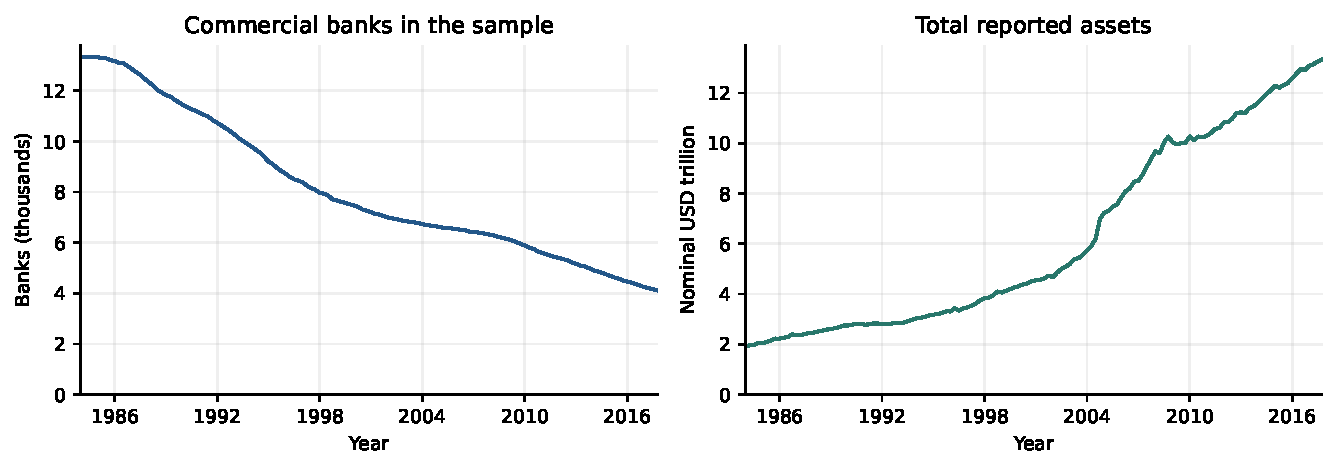
\includegraphics[width=0.92\textwidth]{figures/industry.pdf}
\caption{Commercial-bank counts and summed positive reported total assets.}\label{fig:industry}
\end{figure}
\begin{figure}[H]
\centering
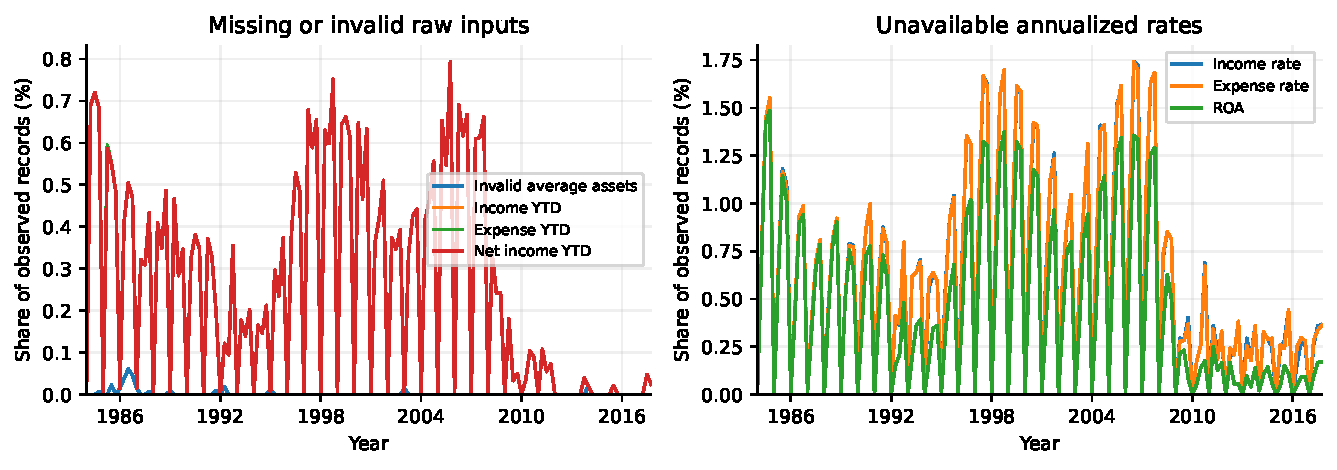
\includegraphics[width=0.92\textwidth]{figures/missingness.pdf}
\caption{Missing or invalid raw inputs and unavailable constructed rates, by quarter. Rates also require quarterly flows and valid assets.}\label{fig:missing}
\end{figure}

\section*{Part 2. Bank-level income and expense betas}
For quarterly flow $Q^y_{it}$ and quarterly average assets $A_{it}$, I construct
\[
 y_{it}=400\frac{Q^y_{it}}{A_{it}},\qquad
 \Delta y_{it}=y_{it}-y_{i,t-1},\qquad
 \Delta f_t=f_t-f_{t-1}.
\]
Rates and changes are in percentage points. Within each bank, I subtract the preceding cleaned rate only when both rates exist and their quarter codes differ by one, including Q4 to Q1. Otherwise the difference is missing. For $f_t$, I retain the supplied March, June, September and December monthly rates and merge them one-to-one onto a 1983Q1--2017Q4 calendar. Duplicate policy quarters, unmatched dates, missing rates, or values outside $[0,100)$ stop execution; this bound is a broad plausibility check in percent units. I construct policy changes and three lags before restricting to 1984Q1--2017Q4. The bank-panel merge is many-to-one by quarter and requires every bank record to match; all four policy regressors are available throughout the analysis period.

For each bank and each outcome, I estimate
\[
 \Delta y_{it}=a_i^y+\sum_{\tau=0}^{3}b^y_{i\tau}\Delta f_{t-\tau}+u^y_{it},
 \qquad \widehat\beta_i^y=\sum_{\tau=0}^{3}\widehat b^y_{i\tau}.
\]
A usable income/expense regression row must have finite values for both outcome changes and all four policy regressors. Both regressions use those same rows. I retain a bank only with at least 40 usable quarters and design-matrix rank five (intercept plus four slopes); the quarters need not be consecutive. The 40-quarter cutoff is arbitrary and pragmatic, not validated as optimal. This leaves an unbalanced sample of \CoreEligible{} banks; \CoreExcluded{} have insufficient observations. Each bank has its own intercept and slopes. Calendar-quarter effects would absorb the common policy regressors. Beta sums only the four slopes, excluding the intercept.

Further investigation is recommended: examine usable history lengths and compare eligibility cutoffs of 20, 40 and 60 quarters, reporting bank coverage, distributions of betas, standard errors and cumulative-response $p$-values, and cross-sectional results. Changing the cutoff changes the eligible sample; estimates for banks retained under every cutoff remain unchanged. Within-bank precision could be investigated separately using different estimation windows. These checks have not been performed, and smaller $p$-values alone do not justify a cutoff.

\begin{table}[H]
\centering
\caption{Distribution and inference for estimated cumulative responses}\label{tab:betas}
\begingroup\small\setlength{\tabcolsep}{4pt}
\begin{tabular}{lrrrrrrrr}
\toprule
 & Banks & Mean & SD & P25 & Median & P75 & \shortstack{Median\\HAC SE} & \shortstack{Significant\\(\%)} \\
\midrule
Income beta & 10,399 & 0.369 & 0.159 & 0.276 & 0.354 & 0.447 & 0.082 & 86.0 \\
Expense beta & 10,399 & 0.356 & 0.104 & 0.298 & 0.352 & 0.410 & 0.052 & 95.7 \\
ROA beta & 10,439 & 0.025 & 0.293 & -0.086 & 0.007 & 0.110 & 0.167 & 2.8 \\
\bottomrule
\end{tabular}

\endgroup
\begin{minipage}{0.94\textwidth}\footnotesize
Equal weight per eligible bank; all estimated betas enter distribution statistics. ROA uses its own available quarters and the same 40-quarter threshold. Units are outcome pp per policy pp. Significant means a two-sided, unadjusted $p<0.05$, regardless of sign. Inference summaries require a finite positive SE, a $p$-value in $[0,1]$, and test status \texttt{ok}; unavailable tests: income \IncUnavailableTests{}, expense \ExpUnavailableTests{}, ROA \RoaUnavailableTests{}.
\end{minipage}
\end{table}

For each bank, I test $H_0:\sum_{\tau=0}^{3}b_{i\tau}=0$ using an asymptotic normal Wald test. Standard errors use Bartlett HAC weights through four actual calendar-quarter lags, the $n/(n-5)$ correction, and all slope covariances; gaps are not compressed into adjacent periods. Constant outcomes or zero/invalid cumulative-response variance receive unavailable tests, not nonsignificant labels. HAC allows heteroskedasticity and serial correlation, but inference can depend on bandwidth and be inaccurate in short samples. Tests are unadjusted for multiple comparisons. These bank-level summaries neither test the cross-bank mean nor establish causal effects.

Mean income and expense betas are \IncMean{} and \ExpMean{}; their medians are \IncMedian{} and \ExpMedian{}. A one-percentage-point permanent rise in the policy-rate level is therefore associated with \IncMean{} pp higher income rates and \ExpMean{} pp higher expense rates after four quarters for the average eligible bank. These are asset-scaled rates, so the expense beta is not a deposit-rate beta. Similar average responses suggest substantial offsetting repricing of income and costs. The estimates are descriptive: policy responds to economic conditions, banks face shared shocks, and bank-specific sample windows differ. The required one-row-per-bank income/expense estimates are in \texttt{bank\_betas.csv}.

\section*{Part 3. Cross-sectional analysis and market data}
\subsection*{A. Income and expense sensitivities}
I estimate $\widehat\beta_i^{Inc}=\alpha+\gamma\widehat\beta_i^{Exp}+\varepsilon_i$ by OLS, giving equal weight to each bank with both betas finite. No beta is trimmed or excluded for its $p$-value. Table~\ref{tab:cross} uses HC3 standard errors, allowing heteroskedasticity and adjusting the variance estimate for leverage, but not first-stage estimation error or common shocks across banks. Bank fixed effects would saturate this one-observation-per-bank regression; there is no common observation date for time effects.

The slope of \IncAllSlope{} means that banks with a one-unit higher expense sensitivity have, on average, a \IncAllSlope{}-unit higher income sensitivity. Equivalently, their predicted income-rate response to a 1 pp policy increase is \IncAllSlope{} pp higher. At zero expense sensitivity, predicted income sensitivity is \IncAllIntercept{}. The positive association is consistent with banks matching asset repricing to funding costs, but does not establish active hedging or a causal effect of funding costs.

Bank size is the arithmetic mean of \texttt{ave\_asset} across that bank's shared income/expense regression quarters. Within each cross-sectional sample, finite positive means determine the median, \$\SizeCutoff{} million here: small banks are at or below it; large banks are above it. Banks without a positive finite size remain eligible for the full regression but not the size split. The income slope is \IncSmallSlope{} for smaller banks and \IncLargeSlope{} for larger banks, suggesting stronger comovement among larger banks. Separate estimates do not test whether the slopes differ. Nominal size and different observation windows complicate this comparison.

\begin{table}[H]
\centering
\caption{Cross-sectional relationships between bank sensitivities}\label{tab:cross}
\begin{tabular}{lrrrrrr}
\toprule
 & \multicolumn{3}{c}{Income beta} & \multicolumn{3}{c}{ROA beta} \\
 & All & Small & Large & All & Small & Large \\
\midrule
Intercept & 0.122 & 0.140 & 0.118 & -0.025 & 0.024 & -0.054 \\
 & (14.36) & (10.83) & (10.23) & (-1.82) & (1.16) & (-2.72) \\
Expense beta & 0.696 & 0.612 & 0.734 & 0.142 & -0.051 & 0.261 \\
 & (30.09) & (16.50) & (24.25) & (3.66) & (-0.83) & (4.95) \\
Banks & 10,399 & 5,200 & 5,199 & 10,399 & 5,200 & 5,199 \\
Adjusted $R^2$ & 0.206 & 0.142 & 0.248 & 0.002 & 0.000 & 0.009 \\
\bottomrule
\end{tabular}

\begin{minipage}{0.97\textwidth}\footnotesize
OLS; HC3 $t$-statistics in parentheses. Small means average assets at or below the analysis-specific median; large means above it. All finite beta pairs are retained. Both analyses have the same paired-bank sample and size cutoff here.
\end{minipage}
\end{table}

\subsection*{B. Interest sensitivity of profitability}
I construct $ROA_{it}=400Q^{NI}_{it}/A_{it}$ using Part 1's quarterly net income and strictly positive finite average assets, allowing losses and clipping rate tails as specified. Each bank's ROA regression uses rows with finite ROA changes and all four policy regressors, independently of its income/expense sample, with the same 40-observation and rank-five rules. This produces \RoaEligible{} ROA betas; \CoreEligible{} banks have finite ROA/expense pairs for the equal-weight cross-section. The mean ROA beta is \RoaMean{} and the median is \RoaMedian{}, much smaller than the gross interest responses.

In $\widehat\beta_i^{ROA}=\alpha+\gamma\widehat\beta_i^{Exp}+\varepsilon_i$, the slope is \RoaAllSlope{}: a one-unit higher expense beta is associated with a \RoaAllSlope{} pp greater ROA response to a 1 pp policy increase. The intercept is \RoaAllIntercept{} at zero expense sensitivity. The relationship is positive among larger banks (slope \RoaLargeSlope{}) and weak among smaller banks (\RoaSmallSlope{}). The full-sample adjusted $R^2$ is only \RoaAllRsq{}, so expense sensitivity explains little profitability heterogeneity. Loan losses, operating costs and noninterest income can offset gross interest repricing.

For sensitivity, I restore rate levels before winsorization, recompute their calendar differences, and repeat the bank and cross-sectional regressions. Charter, missing-value, negative-interest, minimum-history and rank rules remain unchanged. The income slope stays positive (\RawIncSlope{}, $t=\RawIncT$), but the ROA slope changes sign and is imprecise (\RawRoaSlope{}, $t=\RawRoaT$). The profitability relationship is therefore sensitive to extreme observations.

\begin{figure}[H]
\centering
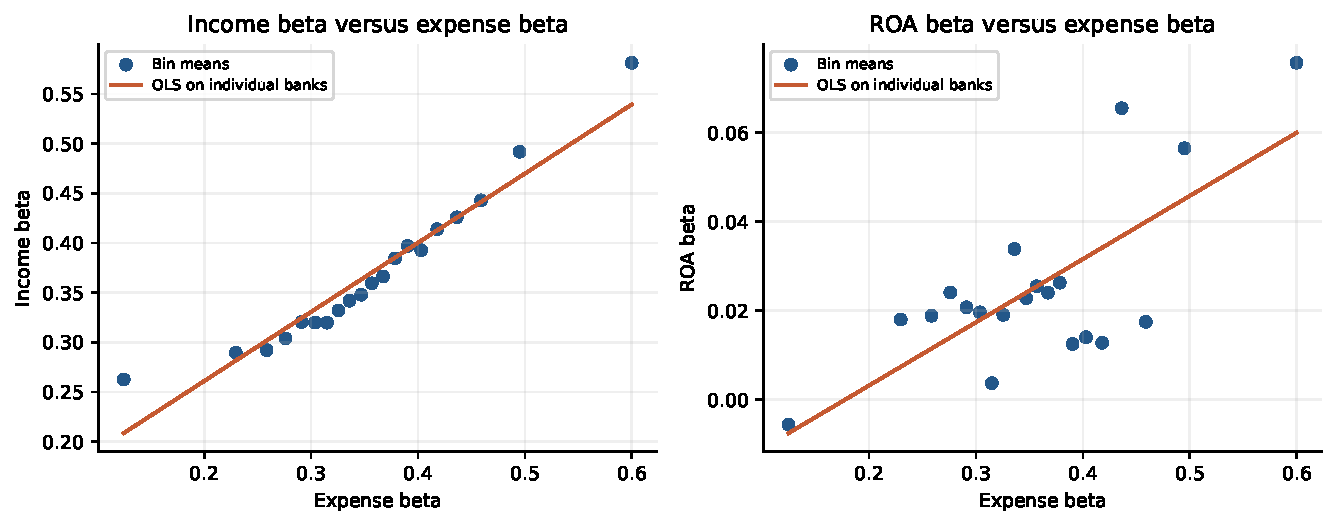
\includegraphics[width=0.92\textwidth]{figures/beta_relationships.pdf}
\caption{All finite beta pairs are grouped into 20 expense-beta quantile bins (ties may reduce the number). Points are equal-weight bin means. Lines fit individual banks, not the bin means, and are displayed over the bin-mean range. No beta outliers are removed.}\label{fig:betas}
\end{figure}

\subsection*{C. Listed companies, share prices and returns}
\textit{Bank-to-company links.} I use all retained commercial-bank quarters, including banks ineligible for beta estimation. After removing identical link rows, a candidate link must satisfy $dt\_start\leq quarter\_end\leq dt\_end$. I match \texttt{idrssd} first, using \texttt{bhc\_id} only if no direct candidate exists. Multiple different \texttt{PERMCO}s at the selected priority cause exclusion, with no fallback from an ambiguous direct match (no such exclusions occur here). Overlapping links to the same company use the latest endpoint. This initially links \LinkedBanks{} banks to \LinkedCompanies{} companies.

\textit{Company accounts.} For every matched bank in a company--quarter, \texttt{total\_asset}, \texttt{ave\_asset}, \texttt{total\_equity} and quarterly \texttt{net\_income\_q} must be finite; both asset measures must also exceed zero. Equity and net income may be negative. If any matched bank fails, the entire company--quarter is excluded (\IncompleteGroups{} groups). I sum the remaining raw dollar amounts by \texttt{PERMCO} and quarter, then calculate
\[
 ROA_{cq}=400\frac{\sum_i NI^q_{iq}}{\sum_i AveAssets_{iq}},\quad
 Capital_{cq}=100\frac{\sum_i Equity_{iq}}{\sum_i TotalAssets_{iq}},\quad
 Size_{cq}=\log\!\left(\sum_i TotalAssets_{iq}\right).
\]
Sums cover matched subsidiaries, and assets are in USD thousands. Across complete company records within each accounting quarter, I clip ROA and capital ratios at their 0.5th and 99.5th percentiles before matching stocks and return months. Bank-level clipped ROA is not aggregated. Completeness concerns the matched banks' fields; it does not establish coverage of every subsidiary or consolidated holding-company accounts.

\textit{Stock records.} The stock-date filter is January 1984--December 2017; the supplied file starts in January 2000. A security record must cover the return month's first day within its classification start/end dates. I require US incorporation (\texttt{USIncFlg=Y}), issuer type \texttt{CORP} or \texttt{ACOR}, security type \texttt{EQTY}, subtype \texttt{COM}, share type \texttt{NS}, and an identified US listing exchange: \texttt{N/A/Q/R/B/I} (NYSE, NYSE American/AMEX, Nasdaq, NYSE Arca, Cboe BZX or IEX). Other or missing exchange codes are excluded.\footnote{Field mapping and ordinary-share classification: \href{https://wrds-www.wharton.upenn.edu/pages/wrds-research/macros/crsp-ciztosiz-macro/}{WRDS CRSP CIZ-to-SIZ documentation}.} Within each \texttt{PERMNO}--month, duplicates must agree on company, return date, both returns, prior capitalization and its date; conflicts stop execution. Keeping one such row removes \StockDuplicates{} duplicates. Both total return (\texttt{MthRet}) and ex-dividend return (\texttt{MthRetx}) must be finite and at least $-1$ in decimal units. Prior capitalization (\texttt{MthPrevCap}) must be finite and positive, with \texttt{MthPrevDt} in exactly the preceding calendar month. There is no upper return cutoff. I combine surviving share classes within \texttt{PERMCO}--month using their prior capitalizations as weights.

\textit{Information timing and link expiry.} Actual filing dates are unavailable, so assumed availability is quarter-end plus 120 calendar days. For each company--month, I select the latest complete report whose assumed availability is strictly before the month's first day. I then require the interval from accounting quarter-end to month-start to be at most 365 days, and the company link to last through month-end. If either check fails, that company--month is dropped, without trying an older report. Each subsidiary's link expires at its recorded endpoint, shortened to the day before a later conflicting company link. For holding-company matches, it is also shortened to the last old-parent quarter-end before a change in reported \texttt{bhc\_id}. The company's expiry is the earliest of its matched subsidiaries' expiries. These conservative rules cannot verify late filings or later data revisions.

Applying these explicit stock, account and timing rules leaves \MarketBanks{} contributing banks, \MarketCompanies{} listed companies and \MarketObservations{} company--months over January 2000--December 2017.

Figure~\ref{fig:prices} chains monthly ex-dividend returns, first within companies and then across the available accounting-linked companies, with the same prior-month capitalization weights. December 1999 equals 100. This produces a comparable price index rather than averaging dollar share prices; it excludes cash dividends and changes composition as firms enter or exit. The series falls sharply during the financial crisis and recovers to \MarketLastIndex{} by December 2017.

\begin{figure}[H]
\centering
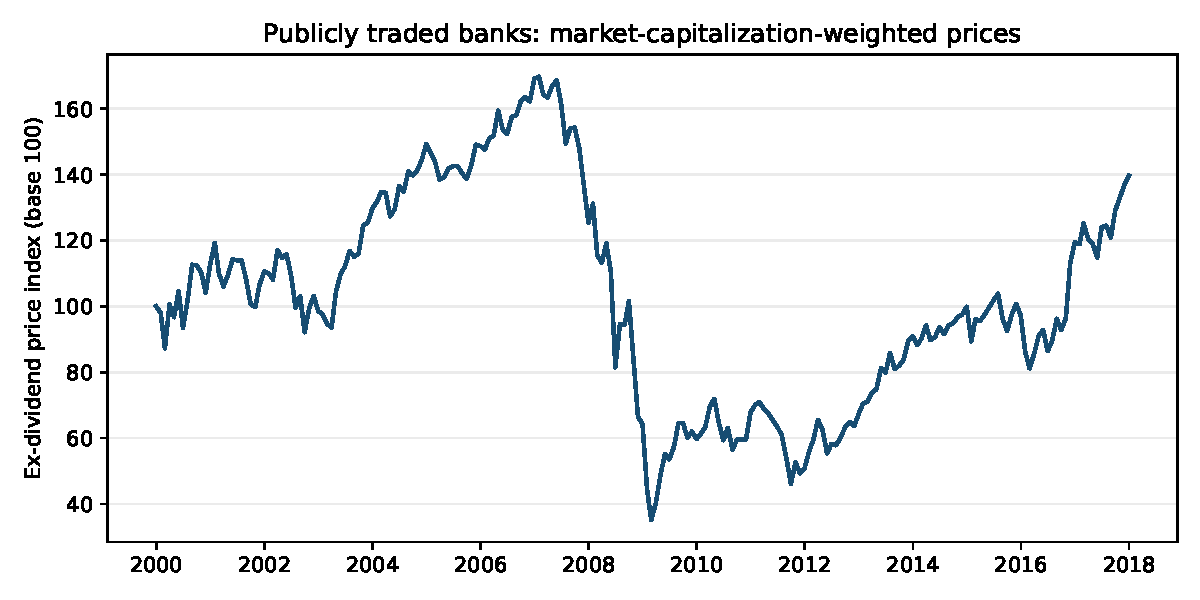
\includegraphics[width=0.80\textwidth]{figures/bank_stock_price_index.pdf}
\caption{Ex-dividend price index for companies with usable prior accounting data. December 1999 = 100.}\label{fig:prices}
\end{figure}

For monthly total stock return $r_{cm}$ in percentage points, I estimate
\[
 r_{cm}=\alpha_c+\lambda_m+\theta_1\log(Assets_{c,q(m)})
       +\theta_2ROA_{c,q(m)}+\theta_3Capital_{c,q(m)}+e_{cm},
\]
where $q(m)$ denotes the latest eligible prior report. Company effects absorb persistent differences; month effects absorb common market movements. Standard errors are clustered by company and month to allow serial and contemporaneous dependence. The coefficients describe within-company associations conditional on common monthly shocks; a separate intercept is absorbed by the fixed effects.

\begin{table}[H]
\centering
\caption{Company characteristics and subsequent monthly stock returns}\label{tab:market}
\begin{tabular}{lr}
\toprule
 & Monthly return (pp) \\
\midrule
Log assets & -0.628 \\
 & (-3.74) \\
Annualized ROA (pp) & 0.034 \\
 & (0.31) \\
Equity/assets (pp) & -0.043 \\
 & (-2.42) \\
Company and month effects & Yes \\
Company-months & 64,230 \\
Companies & 691 \\
Adjusted $R^2$ (including effects) & 0.175 \\
\bottomrule
\end{tabular}

\begin{minipage}{0.85\textwidth}\footnotesize
OLS with company and month fixed effects; $t$-statistics use two-way clustered standard errors. ROA and equity/assets are in percentage points. Assets are measured in nominal USD thousands before taking logs. Adjusted $R^2$ includes the fixed effects.
\end{minipage}
\end{table}

A one-log-unit increase in assets is associated with a \StockSize{} pp change in monthly returns; a 1 pp increase in equity/assets is associated with a \StockCapital{} pp change. Lower capital can coincide with greater leverage and risk compensation, but the estimates do not establish that mechanism. The ROA coefficient is \StockRoa{} pp per 1 pp of ROA and is imprecise. Accounting performance need not predict returns when prices already incorporate it. These are conditional associations, not a trading strategy or causal estimates; reporting delays, incomplete company coverage and changes in risk remain relevant.
\clearpage
\begin{center}\Large Question 2: Policy-rate changes and banks' cash shares\end{center}

\section*{1. Question and motivation}
I ask this question because the relationship between short-term interest rates and cash or reserve holdings is a straightforward mechanism often discussed in introductory monetary and macroeconomics courses. I am interested in how much explanatory power this relationship retains in real markets, where banks face complex conditions and unexpected shocks. Specifically, how much of the quarterly variation in commercial banks' cash-to-assets ratios is associated with current and recent federal funds rate changes during 1984--2017? I use Question 1's bank-specific regression structure and report model fit alongside sensitivity estimates.

\section*{2. Data, construction and estimation}
The only data inputs are \texttt{callreports\_1984\_2017.dta} and \texttt{FedFunds.csv}, both supplied for Question 1. The bank file labels \texttt{cash} as ``Cash and balances due from depository institutions.'' It includes more than reserves at the Federal Reserve; the outcome is therefore a broad cash-and-bank-balances share.\footnote{The corresponding reporting category includes currency, collection items and balances at other banks and the Federal Reserve: \href{https://www.chicagofed.org/banking/financial-institution-reports/fr2644-field-information}{Federal Reserve Bank of Chicago, FR 2644 field information, item 1}. The supplied file's label identifies the variable used here.} Both cash and total assets are reported in nominal USD thousands, so their units cancel in the ratio.

The script applies the following rules in order:
\begin{enumerate}
\item \textit{Keys and dates.} Read \texttt{idrssd}, \texttt{year}, \texttt{qdate}, \texttt{charter\_type}, \texttt{cash} and \texttt{total\_asset}; sort by bank and quarter. Require nonmissing, positive integer bank identifiers, integer quarter codes from 96 to 231 (1984Q1--2017Q4), \(year=1960+\lfloor qdate/4\rfloor\), and unique bank--quarter keys. A failed check stops execution; duplicates are not arbitrarily retained or averaged. These checks pass for \QTwoRawRows{} source rows.

\item \textit{Commercial-bank sample.} Retain rows with \texttt{charter\_type=200}; exclude \QTwoOtherCharterRows{} other or unclassified rows. This leaves \QTwoPanelRows{} rows for \QTwoPanelBanks{} banks. Cash availability is assessed independently of the income, expense and ROA samples from Question 1. Banks need not be listed companies.

\item \textit{Cash share.} Require finite \texttt{total\_asset}>0 and finite \(0\leq cash\leq total\_asset\). Set the ratio to missing if either condition fails, retaining the row for the audit. There are \QTwoInvalidAssetRows{} rows with invalid assets and \QTwoNonfiniteCashRows{} with nonfinite cash; these counts can overlap. There are \QTwoNegativeCashRows{} finite negative cash values and \QTwoCashAboveAssetsRows{} cash values above finite assets; the latter flag is a zero-assets observation already counted as invalid. In total, \QTwoInvalidRatioRows{} ratios are unavailable and \QTwoValidRatioRows{} are usable. Calculate
\[
 c_{it}=100\frac{cash_{it}}{total\_asset_{it}}.
\]
Zero cash and cash equal to assets remain valid. These are quarter-end balance-sheet stocks: use total assets, not quarterly average assets, and apply neither YTD subtraction nor annualization. Unlike Question 1's outcome rates, shares are not winsorized: values inside the accounting bounds are retained. This avoids another arbitrary cutoff, although unusual values within the bounds can still reflect errors.

\item \textit{Quarterly changes.} Within each bank, calculate \(\Delta c_{it}=c_{it}-c_{i,t-1}\) only when both ratios exist and their quarter codes differ by exactly one. Both records must survive the commercial-bank restriction. Q4-to-Q1 changes are allowed; the first record, missing inputs and gaps produce missing changes. Negative changes are valid declines. There is no interpolation, replacement of missing values, or balanced-panel requirement. This leaves \QTwoUnavailableDiffRows{} observed rows without a usable change. With no pre-1984 bank data, estimation starts no earlier than 1984Q2.

\item \textit{Policy rate and merge.} Reuse Question 1's \texttt{f\_construction()}: take the monthly effective federal funds rate in March, June, September and December, in percent. Match one-to-one to a complete 1983Q1--2017Q4 calendar; duplicate quarters, unmatched dates, missing rates or rates outside \([0,100)\) stop execution. Construct \(\Delta f_t=f_t-f_{t-1}\) and its three quarterly lags before restricting to 1984--2017. Left-merge onto bank observations using \texttt{qdate}, requiring many-to-one matching and a policy match for every bank row. The policy calendar is complete; gaps in bank histories never alter policy-lag distances.

\item \textit{Regression eligibility.} Keep rows with finite \(\Delta c\) and all four policy regressors: \QTwoUsableRows{} bank--quarters before the minimum-history rule. Each bank needs at least 40 such observations and design-matrix rank five. Quarters need not be consecutive. The 40-quarter cutoff is inherited from Question 1 and remains arbitrary; no new cutoff search is performed. The audit identifies \QTwoTooFewBanks{} banks with insufficient observations and \QTwoRankDeficientBanks{} remaining banks with deficient rank. Estimate \QTwoEstimatedBanks{} banks using \QTwoEstimationRows{} observations in total.
\end{enumerate}

For each eligible bank, fit ordinary least squares:
\[
\Delta c_{it}=a_i+\sum_{j=0}^{3}b_{ij}\Delta f_{t-j}+u_{it},
\qquad \widehat\beta_i=\sum_{j=0}^{3}\widehat b_{ij}.
\]
Each usable quarter has equal weight within a bank; each estimated bank has equal weight in the summaries. The intercept permits a bank-specific average change. Differencing removes constant differences in cash-share levels. Full calendar-quarter fixed effects would give each date (1984Q1, 1984Q2, and so on) its own intercept. Since each bank has one observation per date, these effects would fit every observation separately and absorb all four policy regressors, leaving their coefficients unidentified. They are therefore omitted. No additional controls, subgroup regressions or cross-sectional second-stage regressions are added.

Beta excludes the intercept and measures the associated cumulative cash-share change over the current and following three quarters for a one-percentage-point policy-rate increase, holding other policy changes fixed. To describe fit, calculate
\[
R_i^2=1-\frac{\sum_t\widehat u_{it}^{\,2}}
 {\sum_t(\Delta c_{it}-\overline{\Delta c_i})^2},
\qquad
\overline R_i^2=1-(1-R_i^2)\frac{n_i-1}{n_i-5}.
\]
The first measures in-sample variation accounted for by the four policy regressors beyond an intercept. The second adjusts for fitting five parameters; negative adjusted values are retained. Neither statistic measures causal explanatory power or forecasting performance.

Inference follows Question 1: Bartlett HAC covariance through four actual calendar-quarter lags, correction \(n_i/(n_i-5)\), and a two-sided asymptotic normal Wald test of \(H_0:\sum_j b_{ij}=0\). The beta variance sums the entire four-by-four slope covariance block, including covariances. A constant outcome or nonpositive/nonfinite beta variance receives unavailable inference; a constant outcome also has unavailable fit statistics. Point estimates remain in the distribution. Median SE and the significant share use only tests with status \texttt{ok}, finite positive SE and \(p\in[0,1]\); significance means \(p<0.05\). Tests are unadjusted for multiple comparisons. This tests the slope sum, not the joint hypothesis that every lag coefficient is zero, and supplies no test of the mean beta across banks.

\section*{3. Evidence}
\begin{table}[H]
\centering
\caption{Bank-level cash-share responses and model fit}
\begin{tabular}{lr}
\toprule
Metric & Value \\
\midrule
Eligible banks & 10,560 \\
Mean cumulative beta & -0.210 \\
Median cumulative beta & -0.158 \\
Median HAC standard error & 0.378 \\
Banks with cumulative $p<0.05$ (\%) & 7.1 \\
Median $R^2$ & 0.046 \\
Median adjusted $R^2$ & -0.003 \\
\bottomrule
\end{tabular}

\begin{minipage}{0.9\textwidth}\footnotesize
Equal bank weights. Beta units are cash-share percentage points per policy-rate percentage point. Median HAC SE is the median uncertainty of individual bank betas, not the SE of the mean or median beta. Significant shares exclude \QTwoUnavailableTests{} unavailable tests. Fit statistics describe quarterly changes, with an intercept in every regression.
\end{minipage}
\end{table}

The mean cumulative beta is \QTwoMeanBeta{} and the median is \QTwoMedianBeta{}. A one-percentage-point policy-rate increase is associated with a cumulative cash-share change of \QTwoMeanBeta{} percentage points for the average eligible bank, under the fitted model. Across banks, the median \(R^2\) is \QTwoMedianRSquared{}: the model accounts for about 4.6\% of within-bank variation in quarterly cash-share changes at the median. Median adjusted \(R^2\) is \QTwoMedianAdjustedRSquared{}, indicating weak fit after accounting for the four policy slopes. The share of available bank tests rejecting a zero cumulative association is \QTwoSignificantShare{}\%. Economic magnitude, model fit and statistical significance address different questions; lag coefficients can offset in the cumulative sum even when they help fit the data.

\begin{figure}[H]
\centering
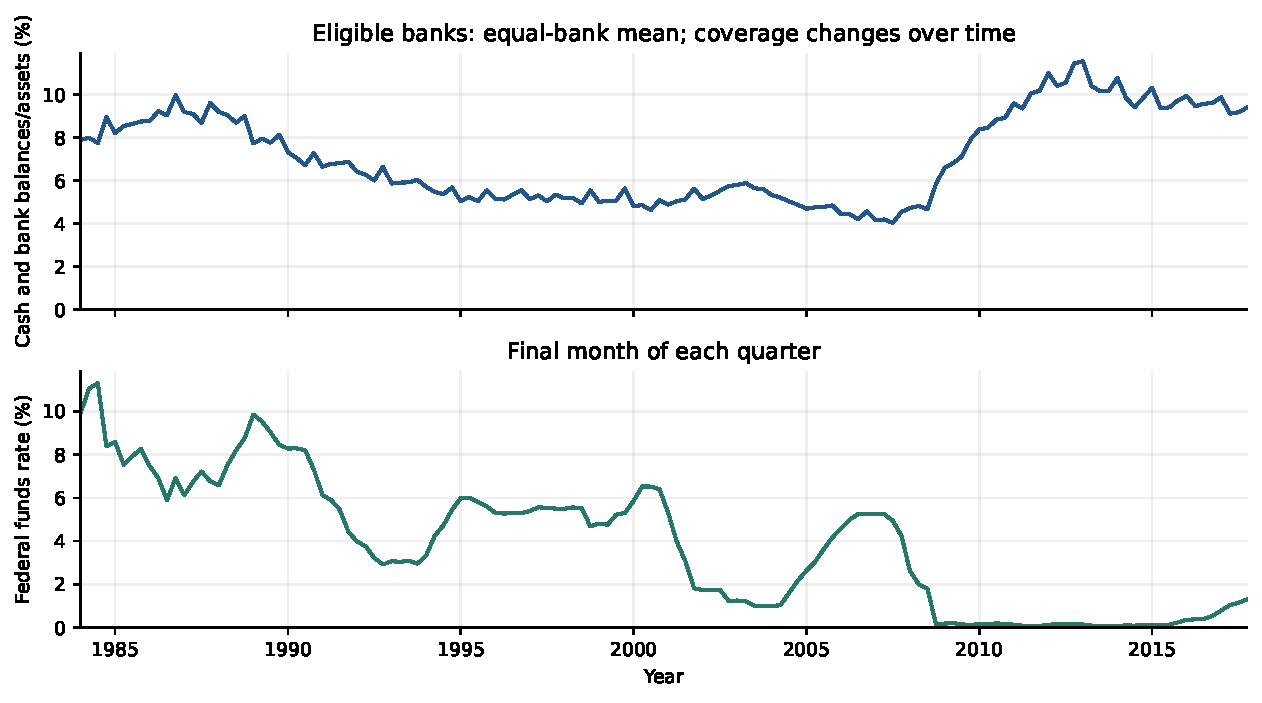
\includegraphics[width=0.82\textwidth]{figures/question2_cash.pdf}
\caption{Cash shares and the federal funds rate. The upper panel averages valid cash shares equally across regression-eligible banks observed in each quarter; the lower panel uses the quarter's final monthly policy rate. The available bank composition changes over time. These level series provide context; the regressions use bank-level changes.}
\end{figure}

The plotted mean cash share is \QTwoFirstMeanCash{}\% in 1984Q1 and \QTwoLastMeanCash{}\% in 2017Q4. This describes available eligible banks, not an asset-weighted industry ratio or the evolution of a fixed bank cohort.

\section*{4. Interpretation and limitations}
The negative average response is consistent with banks reducing their cash share as policy rates rise, but the low fit statistics indicate limited explanatory power. This does not by itself reject the textbook mechanism: the outcome is broader than Fed reserves, and the model describes association rather than an identified policy effect.

I do not control for major macroeconomic events, including recessions and financial crises, which can affect both policy rates and banks' cash holdings. The introduction of interest on reserve balances in October 2008 may also change the relationship over time.\footnote{\href{https://www.federalreserve.gov/newsevents/pressreleases/monetary20081006a.htm}{Federal Reserve announcement, October 6, 2008}.} Nor do I explicitly model banks' different business focuses, such as lending mix, deposit funding and payment services, or changes in those activities. Separate bank intercepts and slopes allow different average changes and estimated responses, but do not explain the sources of those differences or control for changing business conditions.

I also do not construct each bank's minimum required reserves or account for regulatory changes during the sample. Requirements depended on the types and amounts of reservable liabilities, with exemptions, thresholds and ratios that changed over time; banks with different funding structures could therefore face different requirements.\footnote{Federal Reserve \href{https://www.federalreserve.gov/monetarypolicy/rmm/Chapter_3_Calculation_of_Reserve_Balance_Requirements.htm}{Reserve Maintenance Manual} and \href{https://www.federalreserve.gov/monetarypolicy/reservereq.htm}{historical reserve requirements}.} The broad cash/assets ratio is not a measure of compliance with those requirements.

Ratio changes can reflect either cash or total assets; entry, exit, mergers and differing bank histories affect comparability. HAC standard errors address heteroskedasticity and serial correlation, not omitted-variable bias, and may be unreliable with short histories. Nominal significant shares also face multiple-testing concerns and correlated bank outcomes.
\par\smallskip
{\small\textbf{Time spent (reported).} Question 1: Part 1: 20 minutes. Part 2: 1.5 hours. Part 3: 1.5 hours.\quad Question 2: 3 hours.}
\end{document}
